\documentclass[a4paper,11pt,titlepage]{article}    
%\usepackage{tikz} 
\usepackage{graphics}
\usepackage{pdfpages}
\usepackage[francais]{babel}
\usepackage[latin1]{inputenc}
\usepackage[T1]{fontenc}
\usepackage{amssymb}
\usepackage{alltt}
%pdfpagemacro
\newcommand\insExemplePDF[1]{\includegraphics[page=#1]{/Users/aurelien/Desktop/projet3A/fib(3).pdf}}
\newcommand\insPolygraphPDF[1]{\includegraphics[page=#1]{/Users/aurelien/Desktop/projet3A/Polygraph.pdf}}
\newcommand\insModele[2]{\includegraphics[page=#1,angle=#2,scale=0.79]{/Users/aurelien/Desktop/projet3A/PolygraphicProgram.pdf}}
%marges
%preamble
\title{Compilateur pour programmes polygraphiques en TOM}
%Projet de 3\`{e}me ann\'{e}e_Ecole des Mines de Nancy
\author{Aurelien Monot}
% Yves Guiraud et Pierre-Etienne Moreau
\date{15/02/2007}
%document
\begin{document}
%maketitle
\maketitle
%\begin{center}
%Projet de recherche de troisi\`{e}me ann\'{e}e \`{a} l'\'{e}cole des Mines de Nancy effectu\'{e} au LORIA\\
%\textbf{Tuteurs :} \textit{YvesGuiraud} et \textit{Pierre-\'{E}tienne Moreau}
%\end{center}
%abstract
%\begin{abstract}
%a rediger en dernier ?
%\end{abstract}
%Table des matieres
\tableofcontents

\newpage 
%INTRODUCTION
\section{Introduction}
%programmes polygraphiques
\paragraph{Programmes polygraphiques -}
L'une des activit\'{e}s au sein de l'\'{e}quipe Pareo du LORIA consiste \`{a} construire des programmes d'un nouveau type, en se basant sur la structure des polygraphes. En voici un exemple :
\begin{center} 
\insExemplePDF{7}\\\insExemplePDF{8}\end{center}
Ce \textit{programme} permet de calculer l'addition sur les entiers naturels. Par quelle magie ? Tout d'abord, on construit les entiers naturels comme des \textit{circuits} avec \insExemplePDF{1} et \insExemplePDF{2}. Ainsi, on a : 0 = \insExemplePDF{1}, 1= \insExemplePDF{3}, et 2 = \insExemplePDF{4}. Ensuite, il suffit de brancher nombres de notre choix sur les entr\'{e}es de notre fonction addition : \insExemplePDF{5}. Enfin, pour effectuer le calcul, on utilise notre \textit{programme} : les expressions $\Rrightarrow_{i}$ d\'{e}finissent les transformations subies par le circuit lors de l'ex\'{e}cution. Ainsi, si on reconna\^{\i}t un membre gauche d'une de ces expressions, on le remplace par le membre droit correspondant. On continue de calculer en proc\'{e}dant ainsi tant qu'on le pourra pour obtenir le r\'{e}sultat. Essayons donc de calculer 2 + 1 avec ce \textit{programme} : \\
\begin{center}\insExemplePDF{15}\\On obtient bien 3\end{center}
Ces programmes pr\'{e}sentent de nombreux int\'{e}r\^{e}ts du fait de leur structure de polygraphes. Les polygraphes peuvent \^{e}tre vus comme un syst\`{e}me de r\'{e}\'{e}critures pour circuits alg\'{e}briques. Ainsi, certaines de leur propri\'{e}t\'{e}s calculatoire en terme de terminaison, de confluence et de complexit\'{e} ont \'{e}t\'{e} \'{e}tudi\'{e}es (r\'{e}f\'{e}rences...Albert Burroni, Yves Lafont, Yves Guiraud...). Il serait ainsi possible de d\'{e}velopper des nouveaux outils d'analyse de code, dans le but de produire des certificats de qualit\'{e} pour les programmes. On peut \'{e}galement imaginer la conception de processeur d\'{e}di\'{e}s, qui calculent naturellement de fa\c{c}on polygraphique.
%\enonce du projet
\paragraph{Objectifs du projet -} 
Avant cela, on cherche \`{a} construire et ex\'{e}cuter des programmes polygraphiques sur une machine classique. L'objectif du projet donc de participer \`{a} cette concr\'{e}tisation en d\'{e}veloppant un compilateur permettant de programmes polygraphiques. Plus pr\'{e}cis\'{e}ment, le but est de concevoir une structure de donn\'{e}e et des algorithmes pour :
\begin{itemize}
\item \textit{Importer et exporter une repr\'{e}sentation XML des programmes polygraphiques. }
\item \textit{Effectuer les op\'{e}rations de recherche et de remplacement de sous-circuits.}\\
\end {itemize}
% introduction de tom
\paragraph{Tom -}
Tom est un langage de programmation permettant d'ajouter des fonctionnalit\'{e}s de filtrage \`{a} Java (ainsi que d'autres langages de programmation). Ainsi, il constitue un outil id\'{e}al pour mettre en oeuvre les syst\`{e}mes fond\'{e}s sur des r\`{e}gle de r\'{e}\'{e}criture et donc en particulier les programmes polygaphiques. Le choix de l'usage de TOM pour ce projet est donc assez naturel. L'implantation du projet est donc r\'{e}alis\'{e}e en Java \'{e}tendu avec Tom.
%compilateur ou interpreteur?
\paragraph{Interpr\^{e}teur ou compilateur ? -}
On remarquera, que l'\'{e}nonc\'{e} du sujet laisse la libert\'{e} de r\'{e}aliser un compilateur ou un interpr\^{e}teur. Ici, le choix de r\'{e}aliser un compilateur a \'{e}t\'{e} fait. Ce choix semblait plus simple \`{a} mettre en oeuvre. On distinguera ainsi au cours du rapport le fonctionnement du programme produit par le compilateur et la production de ce programme par le compilateur.
%annonce du plan ?
\\\\\indent On reviendra tout d'abord plus en d\'{e}tail sur la structure des programmes polygraphiques. Nous verrons ensuite comment mettre en oeuvre un programme polygraphique avec Tom. Enfin, nous \'{e}tudierons le fonctionnement du compilateur permettant d'obtenir ces programmes en Tom.

%PROGRAMMES POLYGRAPHIQUES
\section{Programmes polygraphiques}
%polygraphes
Un des objectifs du projet, et un pr\'{e}-requis indispensable pour la suite du travail est de mod\'{e}liser la structures des programmes polygraphiques. Pour cela, nous reviendrons sur la structure des polygraphes, nous \'{e}tudierons ensuite les sp\'{e}cificit\'{e}s de nos programmes par rapport aux polygraphes puis \'{e}tablirons le mod\`{e}le utilis\'{e} pour la suite du projet.
\subsection{Polygraphes}
Une fa\c{c}on d'aborder les polygraphes consiste \`{a} les consid\'{e}rer comme un syst\`{e}me de r\'{e}\'{e}criture sur des circuits alg\'{e}briques. On peut aussi penser \`{a} des circuits \'{e}lectriques pour mieux comprendre. On introduit ici successivement les polygraphes de dimension 1 \`{a} 3.\\\\
\paragraph{Types -}
Tout d'abord, il y a les \textit{fils}, appel\'{e}s \textit{1-cellules}. Chaque fil transporte une information d'un type \'{e}l\'{e}mentaire. On construit des types plus complexes en associant plusieurs 1-cellules en formant ainsi un \textit{1-chemin} en mettant en parall\`{e}le plusieurs fils. Voici un exemple de 1-chemin constitu\'{e} d'un triplet de 1-cellules associ\'{e}es respectivement \`{a} un entier natural, une liste et un bool\'{e}en :
\begin{center}\includegraphics[scale=0.7,page=1]{/Users/aurelien/Desktop/projet3A/Polygraph.pdf}\end{center}
Le montage en parall\`{e}le (ou juxtaposition) est not\'{e} $\star_{0}$.
\paragraph{Op\'{e}rations -}
Les \textit{op\'{e}rations} sont repr\'{e}sent\'{e}es par des circuits, appell\'{e}s \textit{2-chemins}. Ils sont orient\'{e}s, habituellement du haut vers le bas. Les op\'{e}rateurs sont repr\'{e}sent\'{e}s par des composants appel\'{e}es \textit{2-cellules}. On compose les 2-chemins ou associant les 2-cellules de deux fa\c{c}ons : soit en les montant en parall\`{e}le (juxtaposition not\'{e}e $\star_{0}$), soit en les montant en s\'{e}rie (connection not\'{e}e $\star_{1}$) : 
\begin{center}\insPolygraphPDF{2}\end{center}
Pour chaque composant, on appelle les fils qui entrent sa \textit{source} et les les fils qui sortent son \textit{but}. Ainsi, on appelle \textit{1-source}(not\'{e} s$_{1}$) et \textit{1-but} (not\'{e} t$_{1}$) les 1-chemins  entrant et sortant d'un 2-cellule (et par extension sortant d'un 2-chemin).
\begin{center}\insPolygraphPDF{4}\end{center}
Comme les sources et buts des 2-cellules sont typ\'{e}s, si on veut connecter deux 2-cellules f et g (f $\star_{1}$ g) comme sur le pr\'{e}c\'{e}dent sch\'{e}ma, cela ne peut se faire que si le 1-but de f est \'{e}gal au 1-source de g.
\\Une particularit\'{e} importante des 2-chemins est que l'on peut repr\'{e}senter une m\^{e}me op\'{e}ration de plusieurs mani\`{e}res. En particulier, s'il est interdit de croiser ou casser des fils, on peut n\'{e}anmoins les \'{e}tirer ou les contracter, ce que l'on peut \'{e}crire graphiquement ou alg\'{e}briquement :
\begin{center}\insPolygraphPDF{3}
$(f \star_{0} s_{1}(g)) \star_{1} (t_{1}(f) \star_{0} g) \equiv f \star_{0} g \equiv (s_{1}(f) \star_{0} g) \star_{1} (f \star_{0} t_{1}(g))$\end{center}
\paragraph{Calculs -}
Enfin, on dispose de \textit{3-chemins} ou \textit{chemins de r\'{e}\'{e}criture}. Ils transforment un 2-chemin donn\'{e} : sa 2-source, en un autre 2-chemin appell\'{e} son 2-but. Ces 3-chemins sonr compos\'{e}es de \textit{3-cellules} correspondant \`{a} des r\`{e}gles de r\'{e}\'{e}criture locales. Pour constituer une 3-cellule (ou r\`{e}gle de r\'{e}\'{e}criture), il est n\'{e}cessaire que sa \textit{2-source} (ou \textit{membre gauche}) et son \textit{2-but} (ou \textit{membre droit}), aient m\^{e}mes 1-source et 1-but.\\Ainsi on peut avoir la 3-cellule F : f $\Rrightarrow$ g \insPolygraphPDF{5}si et seulement si : 
\begin{center}$s_{1}((s_{2}(F))= s_{1}((t_{2}(F))$ \&\&  $t_{1}((s_{2}(F))= t_{1}((t_{2}(F))$ \\$\iff$\\$s_{1}(f)= s_{1}(g)$ \&\&  $t_{1}(f)= t_{1}(g)$\end{center}
On pourrait encore aller plus loin dans la compr\'{e}hension de la structure des polygraphies, mais ce qui a \'{e}t\'{e} pr\'{e}sent\'{e} suffit dans le cadre de ce projet pour introduire les programmes polygraphiques.
%Programmes polygraphiques
\subsection{Programmes polygraphiques}
\paragraph{D\'{e}finition :} Un \textit{programme polygraphique} est un polygraphe particulier de dimension 3. L'ensemble de 2-cellules d'un programme polygrahique se divise en trois cat\'{e}gories distinctes : les \textit{structures}, les \textit{constructeurs} et les \textit{fonctions}. De plus, l'ensemble de 3-cellules d'un programme polygraphique se divise suivant deux cat\'{e}gories : les \textit{r\`{e}gles de structures} et les \textit{r\`{e}gles de fonctions}.
\subsubsection{Constructeurs}On d\'{e}finit l'\textit{arit\'{e}} d'une 2-cellule par la taille (la largeur en nombre de fils) de sa source et sa \textit{coarit\'{e}} par la taille de son but. Les constructeurs sont d\'{e}finis de fa\c{c}on g\'{e}n\'{e}rale comme les 2-cellule avec une coarit\'{e} \'{e}gale \`{a} un. Si on revient \`{a} l'exemple de l'introduction sur les entiers naturels, on avait d\'{e}finit les constructeurs \textit{Zero} : \insPolygraphPDF{9} et \textit{Succ} :  \insPolygraphPDF{10}
\subsubsection{Structures}
\paragraph{Cellules -}
\`{A} chaque 1-celllule, on associe trois structures : un effaceur, une duplication et un croisement. De plus, pour chaque combinaison  de deux types distincts, on associe deux cellules de croisement (une pour chaque sens). Par exemple, si on revient aux entiers naturels, on d\'{e}finit les structures suivantes : \insPolygraphPDF{6}, \insPolygraphPDF{7} et \insPolygraphPDF{8} respectivement pour l'effacement, la duplication et le croisement entre entiers naturels.
\paragraph{R\`{e}gles -}
Ensuite, on associe \`{a} ces structures des 3-cellules de structures d\'{e}finissant des r\`{e}gles de r\'{e}\'{e}critures. On a ainsi autant de 3-cellules que l'on a de combinaisons possibles de constructeurs en entr\'{e}e de structures. Sur les entiers naturels, on aura donc les r\`{e}gles de structures suivantes :
\begin{center}\begin{tabular}{cc}\insPolygraphPDF{11}&\insPolygraphPDF{12}\end{tabular}\end{center}
\begin{center}\begin{tabular}{cc}\insPolygraphPDF{13}&\insPolygraphPDF{14}\end{tabular}\end{center}
\begin{center}\begin{tabular}{cccc}\insPolygraphPDF{15}&\insPolygraphPDF{16}&\insPolygraphPDF{17}&\insPolygraphPDF{18}\end{tabular}\end{center}
\paragraph{Remarque :} on note * le 1-chemin vide.
\subsubsection{Fonctions}
\paragraph{Cellules -} Les fonctions correspondent aux autres 2-cellules. Il n'y a pas de contraintes sur leurs sources et buts. Ils correspondent aux autres op\'{e}rateurs que les structures. Par exemple, on d\'{e}finit sur les entiers naturels les fonctions suivantes : l'\textit{addition}  \insExemplePDF{5} et \textit{fibonacci}   \insExemplePDF{16}. Elles ont le m\^{e}me but mais des sources diff\'{e}rentes.
\paragraph{R\`{e}gles -} Les r\`{e}gles associ\'{e}es aux fonctions correspondent aux r\`{e}gles de calculs. Elles sont au coeur des programmes polygraphiques. Comme pour les structures, elles d\'{e}crivent les transformations \`{a} effectuer lorsque l'on a des constructeurs au voisinage des fonctions (au lieu des structures). Elles sont donc de la forme $C \star_{1} f$ avec $C$ un 2-chemins compos\'{e} de constructeur et $f$ une fonction. Par exemple, pour les deux fonctions introduites au-dessus, on associe les r\`{e}gles suivantes :
\begin{center}\begin{tabular}{cc}\insExemplePDF{7}&\insExemplePDF{8}\end{tabular}\end{center}
\begin{center}\begin{tabular}{ccc}\insExemplePDF{9}&\insExemplePDF{10}&\insExemplePDF{11}\end{tabular}\end{center}
\paragraph{Remarque :} Il a \'{e}t\'{e} choisi de distinguer les cellules de structures des cellules de fonctions utilis\'{e}\'{e}s pour le calcul. En effet, dans les langages de programmations classiques, les permutations, duplications et \'{e}crasements sont fournis via la syntaxe. Ce n'est pas le cas pour les polygraphes. Dans un premier temps, on les distinguera donc des fonctions m\^{e}me si elles ont un fonctionnement similaire.
\subsubsection{Calculs}
Pour effectuer des calculs avec des programmes polygraphiques, on consid\`{e}re un 2-chemin puis on applique tant que possible les r\`{e}gles de r\'{e}\'{e}critures d\'{e}crites par les 3-cellules de fonctins et de structures d\'{e}crites par le programme. On essaie donc de calculer fibonacci(3) avec les \'{e}l\'{e}ments introduits pr\'{e}c\'{e}dement : \\
\begin{center}\insExemplePDF{14}\end{center}
On remarque au passage que l'on peut effectuer plusieurs op\'{e}rations de r\'{e}\'{e}criture d'une \'{e}tape du calcul \`{a} une autre.
%modele choisi
\subsection{Mod\`{e}les utilis\'{e}s}
On construit \`{a} pr\'{e}sent un mod\`{e}le UML des programmes polygraphiques (fig 1). Cela servira de base pour mettre en place les structure de donn\'{e}es qu'on utilisera pour programmer le comportement des programmes polygraphiques (en Tom) et exporter les donn\'{e}es (en XML). On construit au passage un mod\`{e}le UML pour les polygraphes que l'on met en parall\`{e}le avec le premier pour illustrer les liens \'{e}troits entre les deux structures (Fig2).
%modele pour les PP
\begin{figure}\insModele{3}{-90}\caption{Mod\`{e}le UML des programmes polygraphiques}\end{figure}
%Lien entre PP et polygraphes
\begin{figure}\insModele{4}{-90}\caption{Lien entre polygraphes et programmes polygraphiques}\end{figure}
\subsubsection{Retour sur les structures}Comme \'{e}nonc\'{e}, pr\'{e}c\'{e}dement, les cellules de structures sont un peu particuli\`{e}res dans le sens o\`{u} l'on est oblig\'{e} de les explicit\'{e} qu'on on calcul avec des polygraphes de dimension 3 mais qu'elles ont un comportement identique aux cellules de fonction. De plus, on remarque que la connaissance de l'ensemble des 1-cellules utilis\'{e}es dans le programme permet de conna\^{\i}tre toutes les 2-cellules de structures n\'{e}cessaires. Ensuite, la connaissance de l'ensemble des constructeurs utilis\'{e}s dans le programme permet alors de d\'{e}finir de mani\`{e}re syst\'{e}matique les 3-cellules de structure (on reviendra d'ailleurs sur ce point ult\'{e}rieurement). Une id\'{e}e simplificatrice pour la suite du travail, surtout dans le but d'effectuer du filtrage, consiste \`{a} assimiler les 2-cellules de structure au x 2-cellules de fonction. Par contre la distinction constructeur/fonction reste indispensable.
\subsubsection{Gom}
Afin de pouvoir travailler de la mani\`{e}re la plus efficace possible avec Tom, on repr\'{e}sentera les programmes polygraphiques en termes Gom. Gom est un g\'{e}n\'{e}rateur de donn\'{e}es typ\'{e}es. Cela revient \`{a} d\'{e}finir une grammaire pour les programmes polygraphiques. Ainsi, pour le projet, nous utiliserons les termes Gom suivants : 
\begin{alltt}
OnePath = Id()
   | OneCell (Name:String)
   | OneC0 (OnePath*)
	
TwoPath = TwoId (onePath:OnePath)
   | TwoCell (Name:String,Source:OnePath,Target:OnePath,Type:CellType)
   | TwoC0 (TwoPath*)
   | TwoC1 (TwoPath*)

ThreePath = ThreeCell (Name:String,Source:TwoPath,Target:TwoPath)

CellType = Constructor()
   | Function()
\end{alltt}
\paragraph{1-chemins -} Id() repr\'{e}sente le 1-chemin (\textit{OnePath}) vide *. On choisit de d\'{e}finir un type par son nom. Pour cela, on associe un attribut \textit{Name} aux 1-cellules (\textit{OneCells}). On d\'{e}finit $\star_{0}$ sur les 1-chemins \`{a} l'aide de l'op\'{e}rateur $OneC0(OnePath*)$, OnePath* \'{e}tant une liste de 1-chemins. C'est un op\'{e}rateur associatif avec le chemin vide Id() comme \'{e}l\'{e}ment neutre.
\paragraph{Types de cellules -} On d\'{e}finit les deux types de cellules (\textit{CellTypes}) \textit{Constructor} et \textit{Function}, respectivement pour les constructeurs et les fonctions. Comme \'{e}nonc\'{e} pr\'{e}c\'{e}d\'{e}ment, on ne distinguera plus les structures des fonctions pour mener les calculs.
\paragraph{2-chemins -}On choisit de d\'{e}finir une 2-cellule (\textit{TwoCell}) par un nom, sa 1-source,son 1-but et son type, d'o\`{u} les attributs \textit{Name}, \textit{Source} et \textit{Target} de type 1-chemin et le type de type \textit{CellType}. Ensuite, on simule la possibilit\'{e} d'\'{e}tirer des fils avec les termes \textit{TwoId}. Ils correspondent \`{a} la repr\'{e}sentation de leur attribut de type 1-chemin dans l'espace des polygraphes de dimension 2. De fa\c{c}ons similaire aux 1-chemins, on d\'{e}finit sur les 2-chemins (\textit {TwoPaths}) les op\'{e}rateurs $TwoC0(TwoPath*)$ et $TwoC1(TwoPath*)$ respectivement pour les constructions $\star_{0}$ et $\star_{1}$. Ce sont aussi des op\'{e}rateurs associatifs \`{a} \'{e}l\'{e}ment neutre. L'\'{e}l\'{e}ment neutre \'{e}tant la r\'{e}prensation du chemin vide par le terme TwoId() i.e. $TwoId(Id())$.
\paragraph{3-chemins -) Dans le cadre de la programmation polygraphique, on limite les 3-chemins au cas particulier des 3-cellules auxquelles on associe un nom et leurs 2-source et 2-but de fa\c{c}on similaire \`{a} la fa\c{c}on dont on a construit les 2-cellules.
\paragraph{Exemples} \'{e}critures en termes, repr\'{e}sentation graphique et arbre
\subsubsection{XML}
\paragraph{1-Cellules -}
\paragraph{2-Cellules -}
\paragraph{3-Cellules -}
\paragraph{Programmes polygraphiques -}
\section{Reecriture de termes sur les programmes polygraphiques avec TOM}
(fonctionnement du programme g\'{e}n\'{e}r\'{e} par le compilateur)
\\r\'{e}\'{e}criture avec tom
\\Possibilit\'{e} de repr\'{e}senter un m\^{e}me circuit avec plusieurs arbres \'{e}quivalents (*0 et *1)
\subsubsection{Hooks Gom} v\'{e}rifications \`{a} la construction et report des erreurs, v\'{e}rification syntaxique
\subsection{Normalisation}
on ne peut pas avoir de forme unique (reference?) mais on peut le faire assez bien au-dessus des fonctions
\subsection{Gravite}
on fait tomber les constructeurs vers les fonctions
\subsection{regles}
membre gauche=pattern\\membre droit=action\\pb des connections
\subsection{strategies}
comment parcourir un arbre au plus efficace?\\differentes id\'{e}es\\solution retenue
\section{Compilateur}
\subsection{architecture d'un programme polygraphique}
schema xml jusqu'au .class
\subsubsection{partie commune}
normalisation, gravit\'{e}, termes gom,transformations xml vers term et vice-versa
\subsubsection{partie specifique}
ensemble de cellules et de r\`{e}gles
\subsection{Fonctionnement du compilateur}
\subsubsection{generation de la partie commune}
copie de fichiers dans le dossier de destination du programme
\subsubsection{generation de la partie specifique}
au sein du programme final
\begin{itemize}
\item g\'{e}n\'{e}ration des cellules de structures
\item g\'{e}n\'{e}ration des r\`{e}gles de structures
\item transformation des r\`{e}gles en strat\'{e}gies
\item strat\'{e}gie de parcours global
\end {itemize}


\section{Outils d\'{e}velopp\'{e}s en parall\`{e}le}
\subsection{transformation term vers xml et inverse}
classe dans la library (la seule pour l'instant)
\subsection{bibliotheque de fonctions}
nat, list et bool\'{e}enss ainsi que des op\'{e}rations \'{e}l\'{e}mentaires +,/,*,-,and,or,sort,merge,cube,carre,fibonacci,egalit\'{e}s sur listes et entiers
\subsection{generateur de programme.xml}
generation d'un programme polygraphique en XML avec les \'{e}l\'{e}m\'{e}nts sus-mentionn\'{e}s
\subsection{lecture du resultat}
lecture d'un r\'{e}sultat de type nat, list ou bool\'{e}ens s'il ne reste que des constructeurs
\subsection{generateur de tests}
g\'{e}n\'{e}ration d'un ensemble de tests \`{a} partir des \'{e}l\'{e}ments de la biblioth\`{e}que de cellules de base
\\assez facile de changer ou ajouter des tests
\\g\'{e}n\'{e}ration d'un programme qui effectue les tests (cod\'{e}s en xml) sur un programme cible


\section{Conclusion}
\subsection{points-cl\'{e}s}
\begin{itemize}
\item tom parfaitement adapt\'{e}
\item plusieurs formes polygraphiques donc normalisation
\item generation des cellules et regles de structures
\item generation des regles de reecritures en TOM
\end{itemize}
\subsection{ouverture}
\begin{itemize}
\item representation graphique : travaille de GB avec des pointeurs et blender
\item editeur graphique pour eclipse en utilisant GMF a partir du metamodele pr\'{e}sent\'{e}
\item garder la biblioth\`{e}que de base pour la proposer lors de la cr\'{e}ation d'un programme (attention, ajouter des fonctions inutiles ralentit l'ex\'{e}cution du programme)
\item TPDB : grande biblioth\`{e}que de tests, convertir les exemples automatiquement en programme polygraphique ??
\end{itemize}

\end{document}
